\section{Bibliothek}

Die Bibliothek ist sehr wichtig für Studierende: 
Man findet dort Lehrbücher, Monographien und Journals die man zum Studium braucht.
In der Bibliothek Naturwissenschaften am Campus Riedberg könnt ihr
die Lehrbücher für Physik und Mathematik ausleihen,
aber auch die für die Fachbereiche Geowissenschaften, Biowissenschaften,
Biochemie, Chemie und Pharmazie.

Die Lehrbücher für die Grundvorlesungen (alle Pflichtmodule im Bachelor) sind in Semesterstärke vorhanden.
Das bedeutet, jeder Studierende kann ein Exemplar ausleihen
und bis Ende des Semesters behalten.
Diese Bücher sind extra gekennzeichnet -- mit einem grünen Aufkleber -- und können nur Mo-Fr 8:00-18:00 ausgeliehen werden.
Bücher aus der normalen Lehrbuchsammlung könnt Ihr ohne
Vorbestellung in Selbstbedienung ausleihen. 
Die Leihfrist beträgt 4 Wochen, eine Verlängerung ist nicht möglich.

Neben der Lehrbuchsammlung gibt es noch die sogenannte \glqq RVK\grqq  (Regensburger Verbundsklassifikation) Sammlung. Sie befindet sich weiter hinten in der Bibliothek und besteht aus Büchern zu spezielleren Themen, die über die normalen Lehrveranstaltungen hinausgehen. Hier findet ihr alles von Supersymmetrie bis Wolkenphysik oder Materialwissenschaften. Die Bücher in diesem Bereich sind alle nur in kleiner Stückzahl vorhanden (1-4). Meist gibt es zwei Exemplare, eins ist ausleihbar und eins ist Präsenzbestand sodass es immer vor Ort benutzt werden kann. Diese Bücher tragen ein großes gelbes Schild auf dem Buchrücken, auf denen \glqq nicht ausleihbar\grqq steht (ist klar, oder?). Die RVK-Sammlung wird für euch wahrscheinlich erst später im Studium interessant wenn ihr Spezialvorlesungen hört, in denen Profs mit Vorliebe ihr eigenes Buch als Literatur angeben oder wenn ihr spezielle Literatur für eure Abschlussarbeiten braucht. Klolektüre lässt sich hier auch gut finden. 
Die Bücher in dieser Sammlung sind ebenfalls ausleihbar für 4 Wochen, können allerdings bis zu 5 Mal um jeweils 4 Wochen verlängert werden, sofern es keine Vormerkung eines anderen Schwei... ähm Nutzers gibt.

Die dritte große Kategorie an Schriften in der Bibliothek sind die Zeitschriften. Weil sich das ein bisschen zu sehr nach Blitz-Illu und Bunte anhört nennen Wissenschaftler sie aber meistens Journals. Hier werden keine Kuchenrezepte und Diättipps veröffentlicht, sondern wissenschaftliche Abhandlungen, meistens \glqq paper\grqq genannt. Die Journals sind im oberen Stockwerk der Bibliothek zu finden und sind alphabetisch nach Titel sortiert. Hier kann man stundenlang nach dem richtigen suchen, da leider nicht immer nach dem ersten Wort des Titels sortiert wird. Droht ihr euch dort zu verlaufen, fragt einfach an der Theke nach. Die Bibliotheksmitarbeiter haben hier auch oft ihre Probleme aber mit etwas Glück, finden sie schneller, was ihr sucht. 
Zeitschriften sind generell nicht ausleihbar. Fast alle Journals gibt es auch online. Ihr könnt sie lesen falls die Uni ein Abo des passenden Journals hat. Hierzu müsst ihr euch mit eurem Bibliotheksaccount auf der Seite des Journals anmelden. Falls ihr keinen Zugang bekommt weil die Uni nicht genug an die Hu... vom Verlag zahlt gibt es eine hilfreiche Website, die wir euch natürlich nicht offiziell empfehlen dürfen. Nur so viel dazu. Sie fängt mit Sci an und hört mit hub auf, alles dazwischen müsst ihr selbst rausfinden.

Neben Büchern gibt es in der Bibliothek auch Gruppenarbeitsräume und einen Computerraum, in dem man arbeiten kann. Beide sind von der Bibliothek räumlich getrennt und auch außerhalb der Öffnungszeiten der Bibliothek geöffnet. Sie sind beide nur für Studierende geöffnet. Für die Gruppenarbeitsräume muss an der Theke der Bib ein Schlüssel ausgeliehen werden. Der Computerraum kann mit der Goethe-Card geöffnet werden.

Du belegst als Nebenfach Sozialwissenschaften, brauchst das eine Buch aus der Zentralbibliothek aber an der UBahn wird mal wieder gebaut und du hast wirklich gar keinen Bock, mit dem Ersatzbus bis nach Bockenheim zu fahren? Bücher aus der Zentralbibliothek können in (fast) jeden Standort der Bib bestellt und dann abgeholt werden. Auch wenn ihr ein Buch aus der BNat in einer anderen Bibliothek abgeben möchtet ist das kein Problem. Auch hier gilt: Man kann Bücher aus fast jeder Bibliothek in fast jeder anderen abgeben. Schwierig wird es immer wenn es sich um folgende Bibliotheken handelt: Mathe, Informatik, Sport.

Falls ein Prof ein Buch empfiehlt, das absolut klausurrelevant und unerlässlich ist, das die Bib aber nicht besitzt oder das es nicht am Riedberg gibt, keine Panik. Du musst nicht direkt die 5 Euro, die nach Miete noch von deinem Bafög übrig sind sparen, um dieses Buch zu kaufen. Es gibt auf der Website der Bibliothek den Kaufvorschlag. Die Bibliothek ist immer dankbar für Vorschläge und fast alles, was vorgeschlagen wird, wird auch zeitnah angeschafft. Solange es halbwegs sinnvoll ist. Ihr bekommt eine Nachricht sobald das Buch verfügbar ist und es wird direkt für euch reserviert. Ihr könnt es dann einfach an der Theke abholen und euer restliches Bafög in Schokolade anlegen.

Solltest du ein Buch zu spät abgegeben haben, macht die Uni leider direkt Auge. die Gebühren sind bei $\frac{3 Euro}{Buch*Woche}$ und können an der Theke bezahlt werden (\textbf{nur bis 18:00 Uhr}). Bei 12 Euro Schulden bei der Bib oder mehr könnt ihr erstmal keine neuen Bücher mehr ausleihen. Ganz wichtig ist: wenn ihr ein Buch abgebt werden die Mahngebühren eingefroren. Ihr könnt sie einfach später zahlen. Wenn ihr das aber zu lange nicht macht ($\geq 6 Monate$) wird ebenfalls eure Goethe Card für Ausleihen gesperrt, auch wenn ihr weniger als 12 Euro offen habt. Wir empfehlen immer, die Gebühren an der Theke zu zahlen (nur in Bar und \textbf{bis 18:00 Uhr}), da es bei der Überweisung viel Zeit in Anspruch nimmt bis sie an der richtigen Stelle verbucht wird. \par

Das war meine (Janika, Fachschaftlerin und Hiwi in der Bibliothek) kleine schriftliche Bibliotheksführung. Am Anfang des Semesters veranstaltet die Bibliothek aber immer \glqq richtige echte \grqq Führungen. Es empfiehlt sich sehr, so eine Führung mitzumachen. Dort bekommt ihr nochmal alles ganz genau gezeigt, ihr lernt die Räumlichkeiten und das Bibliothekspersonal kennen und ihr könnt Fragen stellen. Außerdem lernt ihr, wie man die Website der Bibliothek benutzt und wie man im Bibliothekssystem Recherchen durchführt, das ist nämlich nicht ganz trivial.
Aber das wichtigste was ihr euch immer merken solltet: \textbf{DIE SEMESTERAUSLEIHE UND MAHNGEBÜHREN BEZAHLEN GEHT NUR BIS 18:00 UHR!!!11!!elf!}



\begin{minipage}{0.5\textwidth}
\noindent
\textbf{Öffnungszeiten:}\\\\
Montag - Freitag 08.00 - 20.00 Uhr\\
Samstag 10.00 - 16.00 Uhr\\


\noindent
\textbf{Ausleihzeiten Semesterausleihe und Mahngebühren:}\\
Montag - Freitag  08.00 - 18.00 Uhr\\


\noindent
\textbf{Öffnungszeiten der Gruppenarbeitsräume:}\\
Montag - Freitag  08.00 - 22.30 Uhr\\
Samstag und Sonntag 10.00 - 19.00 Uhr\\


\noindent
\textbf{Internetadressen:} 
\begin{itemize}
   \item{Bibliothek Naturwissenschaften:}\\
    http://www.ub.uni-frankfurt.de/bnat/home.html
   \item{Universitätsbibliothek:}\\
      http://www.ub.uni-frankfurt.de/
\end{itemize}

\end{minipage}
\begin{minipage}{0.5\textwidth}
 \begin{center}
  %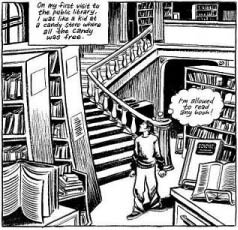
\includegraphics[height=7 cm]{bilder/manga.jpg}
  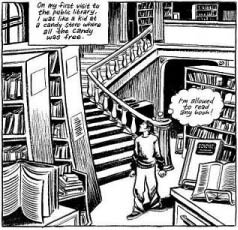
\includegraphics[height=7 cm]{bilder/manga.jpg}
\end{center}
%\vspace*{4cm}
\end{minipage}
\von{Margret}

